
Analog zur Folge definieren wir die (reellwertige) \textit{Funktionsfolge} eine Abbildung $\N \to \R^D$ \quad $ n \mapsto f(n)$. \\
Wir bezeichnen $f(n)$ als $f_n$ (n-te Folge) und die Funktionsfolge mit $\funcsequence$. \\
Für jedes $x \in D$ erhält man eine Folge $(f_n (x))_{n \geq 0}$ in $\R$. ($D$: Menge)
\begin{definition}{Punktweise Konvergenz}\\
    Die Funktionsfolge $\funcsequence$ \emph{konvergiert punktweise} gegen die Funktion $f:D \to \R$, falls für alle $x \in D$: $f(x) = \lim_{n \to \infty} f_n (x)$.
\end{definition}
\noindent\emph{Nur weil eine Funktionsfolge $\funcsequence$ stetig ist, ist die dazugehörige Funktion $f$ nicht unbedingt stetig.}
\begin{example}
    Sei $D= [0,1]$ und $f_n: [0,1] \to \R, n \in \N$\quad $x \mapsto x^n$. Dann folgt:
    \begin{equation*}
        \lim_{n \to \infty} f_n (x) = \lim_{n \to \infty} x^n = 0 \quad \forall 0 \leq x < 1 \qquad f_n (1) = 1
    \end{equation*}
    Also konvergiert die Funk.folge punktweise gegen die Funktion $f: [0,1] \to \R$ gegeben durch:
    \begin{center}
        \begin{minipage}{0.48\linewidth}
            \begin{equation*}
                f(x) = \begin{cases}
                    0 & 0 \leq x < 1\\
                    1 & x = 1
                \end{cases}
            \end{equation*}
        \end{minipage}
        \hfill
        \begin{minipage}{0.48\linewidth}
            Bemerke: Die Funktionen $f_n$ sind alle stetig in $[0,1]$, die Funktion $f$ ist nicht stetig in $1$.
        \end{minipage}
    \end{center}
\end{example} 
\begin{definition}{Gleichmässige Konvergenz $\varepsilon$-Def.}\\
    Die Folge $f_n : D \to \R$ \emph{konvergiert gleichmässig} in $D$ gegen $f: D \to \R$ falls gilt. $\forall \varepsilon > 0~\exists N \geq 1$, sodass
    \begin{equation*}
        \forall n \geq N, \forall x \in D: |f_n (x) - f(x)| < \varepsilon
    \end{equation*}
    Für Funktionenfolgen: $\forall n,m \geq N$ und $\forall x \in D: |f_n(x) -  f_m(x)| < \varepsilon$
\end{definition}
\begin{theorem}{Konvergenz und Stetigkeit}
    Sei $D \subseteq \R$ und $f_ N D \to \R$ eine Funktionsfolge aus (in $D$) stetigen Funktion (in $D$) gleichmässig gegen die Funktion $f:d \to \R$ konvergiert. Dann ist $f$ (in $D$) stetig.
\end{theorem}
\begin{definition}{Gleichmässige Konvergenz Limes-Def.} 
    Eine Funktionsfolge $f_n : D \to \R$ ist \emph{gleichmässig konvergent}, falls für alle $x \in D$ der Grenzwert $f(x) \coloneqq \lim_{n \to \infty} (x)$ existiert und die Folge $\funcsequence$ gleichmässig gegen $f$ konvergiert.\\
    Falls $f_n$ eine gleichmässig konvergente Folge stetiger Funktionen ist, dann ist die Funktion $f(x) \coloneqq \lim_{n \to \infty} f_n (x)$ stetig.
\end{definition}
\begin{definition}{Konvergenz Funktionenreihen}
    Die Reihe $\sum_{k=0}^\infty f_k(x)$ konvergiert gleichmässig (in $D$), falls die durch $S_n (x) \coloneqq \sum_{k=0}^n f_k (x)$ definierte Funktionsfolge gleichmässig konvergiert 
    und deren Grenzwert $f(x) \coloneqq \sum_{n=0}^\infty f_k(x)$
    ist eine stetige Funktion.
\end{definition}
\begin{KR}{Strategie Konvergenz von Funktionenfolgen}\\
    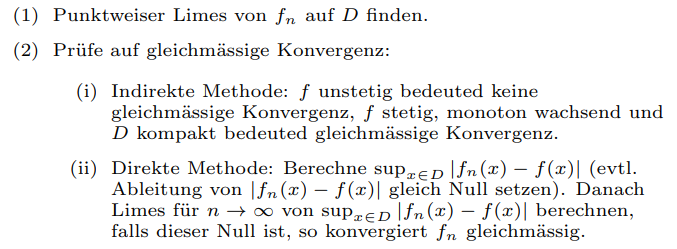
\includegraphics[scale=0.5]{Analysis1/zsf/Images/Stetige_Funktionen/strategie_konvergenz_funktionenfolgen.png}
\end{KR}
